\documentclass[times, 11pt, a4paper]{article}
\usepackage{authblk}
\usepackage{lineno}
\linenumbers

\usepackage[utf8]{inputenc} %unicode support
\usepackage{amsmath}
%\usepackage[applemac]{inputenc} %applemac support if unicode package fails
%\usepackage[latin1]{inputenc} %UNIX support if unicode package fails
\usepackage{todonotes}
\usepackage{caption}
\usepackage{subcaption}
\usepackage{amssymb}
\DeclareCaptionLabelFormat{r-parens}{\textbf{#2}}
\captionsetup[subfigure]{font={bf,small}, skip=1pt, singlelinecheck=false, labelformat=r-parens}
\usepackage{graphicx}
\usepackage{natbib}
\bibliographystyle{plainnat}
\usepackage{hyperref}
\renewcommand{\refname}{REFERENCES}
\renewcommand\Authfont{\fontsize{10}{11}\selectfont}
\renewcommand\Affilfont{\fontsize{9}{11}\emph{\selectfont}}
\usepackage{spverbatim}
\begin{document}

\providecommand{\keywords}[1]{\textbf{Keywords:} #1}

\title{\Large Mapping of RNA modifications by direct Nanopore sequencing and JACUSA2}

\date{}
\author[1,2]{Amina Lemsara}
\author[1,2,3]{Christoph Dieterich\thanks{Correspondence to: christoph.dieterich@uni-heidelberg.de}}
\author[1,2,3]{Isabel Naarmann-de Vries}



\affil[1]{Klaus Tschira Institute for Integrative Computational Cardiology, University  Heidelberg, 69120 Heidelberg, Germany}
\affil[2]{Department of Internal Medicine III (Cardiology, Angiology, and Pneumology), University Hospital Heidelberg, 69120 Heidelberg, Germany}
\affil[3]{German Centre for Cardiovascular Research (DZHK)-Partner Site Heidelberg/Mannheim, 69120 Heidelberg, Germany}

\maketitle

\begin{abstract} % abstract
RNA modifications exist in all kingdom of life. Several different types of base or ribose modifications are now summarized under the term the "epitranscriptome". With the advent of high-throughput sequencing technologies much progress has been made in understanding RNA modification biology and how these modifications can influence many aspects of RNA life. The most widespread internal modification on mRNA is m6A, which has been implicated in physiological processes as well as disease pathogenesis. Here, we provide a workflow for the mapping of m6A sites using Nanopore direct RNA sequencing data. Our strategy employs pairwise comparison of base calling error profiles with JACUSA2. We outline a general strategy for RNA modification detection on mRNA and describe two specific use cases on m6A detection in detail. \textbf{Use case 1:} a sample of interest with modifications (e.g. "wild type" sample) is compared to a sample lacking a specific modification type (e.g. "knock out" sample, here \emph{METTL3}-KO) or \textbf{Use case 2:} a sample of interest with modifications is compared to a sample lacking all modifications (e.g. \emph{in vitro} transcribed cDNA). We provide a detailed protocol on experimental and computational aspects. Extensive online material provides a snakemake pipeline to identify m6A positions in mRNA and to validate the results against  a miCLIP-derived m6A reference set. The general strategy is flexible and can be easily adapted by users in different application scenarios. 
\end{abstract}
\clearpage
%\keywords{Base calling, Nanopore, m6A}

\section*{INTRODUCTION}
Chemical modifications on DNA and histones, also known as epigenetics marks, strongly impact gene expression during cell differentiation and in several other biological programs. In the 1970s, it was recognized that RNA is also subjected to extensive covalent modification, and studies in the late 1980s revealed the widespread deamination of bases (termed RNA editing), which can lead to recoding if it occurs within coding sequences. Impressive development in the RNA modification field occurred during the past eight years, with the discovery of an extensive layer of base modifications in mRNAs. These can influence gene expression and have been already shown to be involved in primary cellular programs such as stem cell differentiation, response to stress, and the circadian clock. The study of RNA modifications and their effects is now referred to as epitranscriptomics, and it reveals striking similarities to what is known for epigenomics.
To date thirteen distinct modifications have been identified on mRNA transcripts \citep{Anreiter2021}. These modifications are catalyzed by a variety of dedicated enzymes and can be divided into two classes: modifications of cap-adjacent nucleotides and internal modifications. 

In contrast to the m7G cap, the impact of internal modifications on gene regulation has been less studied apart from RNA editing, which is mediated by RNA deaminases (e.g. the ADAR family). The most widespread internal mRNA modification is N6-methyladenosine (m6A). By modulating the processing of mRNA, m6A can regulate a wide range of physiological processes and its alteration has been linked to several diseases \cite{Roignant2017,Zaccara2019,Shi2019}. The modification is catalyzed co-transcriptionally by a Mega-Dalton methyltransferase complex, which includes the heterodimer METTL3-METTL14 and other associated subunits \cite{GarciasMorales2021}. This modification is reversible since two proteins of the AlkB-family of demethylases can remove m6A from mRNA transcripts \citep{Jia2011,Zheng2013}. In mammals, m6A preferentially localizes within long internal exons and at the beginning of terminal exons at so-called DRACH motif (D = A/G/U, R = A/G, H = A/C/U) sites \citep{Dominissini2012,Meyer2012,Ke2015}. Once deposited, m6A is recognized by several reader proteins that can affect the fate of mRNA transcripts in nearly every step of the mRNA life cycle, including alternative splicing \citep{Adhikari2016,Roundtree2017}, mRNA translation \citep{wang2015n6} and decay \citep{wang2014n,du2016ythdf2,Roundtree2017}. The best-described readers are the YTH domain family of proteins that decode the signal and mediate m6A functions. By affecting RNA structure, m6A can also indirectly influence the association of additional RNA-binding proteins (RBPs) and the assembly of larger messenger ribonucleoprotein particles (mRNPs) \citep{patil2018reading}.

Several approaches have been presented to map RNA modifications on RNA. Herein, we focus on mRNA modification site detection in general and on m6A in particular where antibody-based protocols (miCLIP), methylation-sensitive restriction enzyme assays (MazF) or transgenic approaches (TRIBE, DART) have been presented to map m6A sites. All of the aforementioned approaches rely on high-throughput short read sequencing on the Illumina platform. This typically involves cDNA synthesis by reverse transcription and PCR-based library amplification. One recent addition to the toolbox of RNA modification mapping is direct RNA single molecule long read sequencing on the Oxford Nanopore Technologies platform (dRNA-seq). While our software is able to deal with Illumina and Nanopore-based approaches, the latter is the principal topic of this methods article.

\section*{MATERIALS}

\subsection*{ONT direct RNA sequencing}
This section summarizes all necessary consumables for direct RNA sequencing of poly-adenylated RNA (i.e. mRNA) on the MinION or similar device.
\begin{enumerate}
\item 500 ng polyA\textsuperscript{+} RNA isolated from total RNA e.g. with Oligotex mRNA kit (\#70022, Qiagen) or Dynabeads oligo dT\textsubscript{25} beads (\#61002, Thermo Fisher Scientific) or \emph{in vitro} transcriptome sample. Store RNA at -80 $^{\circ}$C and the mRNA purification kit as recommended by the manufacturer.

\item Nuclease-free water. Store at room temperature.

\item Direct RNA-sequencing kit (SQK-RNA002, Oxford Nanopore Technologies). Store at -20 $^{\circ}$C.

\item NEBNext Quick Ligation Reaction Buffer (\#B6058S, New England Biolabs). Store at -20 $^{\circ}$C.

\item T4 DNA Ligase (\#M0202S, New England Biolabs). Store at -20 $^{\circ}$C.

\item dNTP Mix (10 mM each, \#R0191, Thermo Fisher Scientific). Store at -20 $^{\circ}$C.

\item SuperScript IV Reverse Transcriptase (\#18090010, Thermo Fisher Scientific). Store at -20 $^{\circ}$C.

\item Agencourt RNAClean XP beads (\#A63987, Beckman Coulter). Store at 4 $^{\circ}$C.

\item 70 \% ethanol, freshly prepared. 

\item Qubit dsDNA HS assay kit (\#Q32854) and Qubit Fluorometer (Thermo Fisher Scientific).

\item Flow cell priming kit (EXP-FLP002, Oxford Nanopore Technologies). Store at -20 $^{\circ}$C.

\item Thermocycler.

\item Gentle rotator mixer.

\item Magnetic stand for 1.5 ml tubes.

\item 1.5 ml DNA LoBind tubes (Eppendorf), 0.2  ml PCR tubes.

\item MinION or GridION sequencing device and MinION R9.4.1 Flow cells (FLO-MIN106D, Oxford Nanopore Technologies). Store Flow cells at 4 $^{\circ}$C.
\end{enumerate}

\subsection*{Preparation of an \emph{in vitro} transcriptome sample}
\begin{enumerate}
\item 100 ng polyA\textsuperscript{+} RNA isolated from total RNA e.g. with Oligotex mRNA kit (\#70022, Qiagen) or Dynabeads oligo dT\textsubscript{25} beads (\#61002, Thermo Fisher Scientific). Store RNA at -80 $^{\circ}$C and the mRNA purification kit as recommended by the manufacturer

\item 10 $\mu$M oligo(dT)-VN RT primer. 

TTTTTTTTTTTTTTTTTTTTTTTTTTTTTTVN. Store at -20 $^{\circ}$C.

\item 20 $\mu$M template switching oligo (TSO). ACTCTAATACGACTCACTATAGGGAGAGGGCrGrG+G. Store at -20 $^{\circ}$C.

\item 10 $\mu$M T7 extension primer. GCTCTAATACGACTCACTATAGG. Store at -20 $^{\circ}$C.

\item Nuclease-free water. Store at room temperature.

\item dNTP Mix (10 mM each, \#R0191, Thermo Fisher Scientific). Store at -20 $^{\circ}$C.

\item Template Switching RT Enzyme Mix (\#M0466S, New England Biolabs). Store at -20 $^{\circ}$C.

\item Q5 Hot Start High-Fidelity 2X Master Mix (\#M0494S, New England Biolabs). Store at -20 $^{\circ}$C.

\item RNase H (5,000 U/ml) (\#M0297S, New England Biolabs). Store at -20 $^{\circ}$C.

\item NucleoSpin Gel and PCR Clean‑up, Mini kit for gel extraction and PCR clean up (\#740609.50, Macherey-Nagel) or equivalent. Store at room temperature.

\item MEGAscript T7 transcription kit (\#AM1334, Thermo Fisher Scientific). Store at -20 $^{\circ}$C.

\item RNA Clean \& Concentrator-25 kit (\#R1017, Zymo Research). Store at room temperature.

\item Thermocycler.

\item Table top centrifuge for 1.5 ml tubes.

\item Nanodrop spectrophotometer or equivalent.

\item 0.2  ml PCR tubes, 1.5 ml DNA LoBind tubes (Eppendorf).

\end{enumerate}

\subsection*{Hardware requirements}
All analyses have been performed/tested on two alternative hardware systems:
a standard Linux desktop computer or an Apple iMac (Retina 5K, ultimo 2014).
The workflow requires a multi-core processor system with minimal main memory of 16GB RAM
and several GBs of free disk space (depending on data set size).

\subsection*{Software dependencies and installation}
Our analysis workflow has few requirements, which are detailed in Table 1. Specifically, to execute our workflow, the following prerequisites are necessary: a BASH shell, a JAVA runtime environment, a working PERL and R installation. Additional i.e. non-standard software to process and map Nanopore reads (bedtools, samtools and Minimap2) are obligatory. Table 2 lists some additional R packages, which are required to run the R code. Detailed instructions on how to setup are found under \url{https://github.com/dieterich-lab/MiMB_JACUSA2_chapter}.

\section*{METHODS}
Our workflow is based on the pairwise comparison of samples with different modification status (Figure \ref{fig:graphicsummary}). The sample of interest (yellow) may be compared to different samples lacking certain modifications. If available, the wild type (WT) sample can be compared to a knock out (KO) sample lacking specific enzymatic activities (green), as outlined in Use Case 1. Alternatively, a sample lacking all modifications may be used for comparison (blue). This may be either a simulated sample (i.e. with NanoSim) or an \textit{in vitro} transcribed sample derived from cDNA. Such an analysis is detailed in Use Case 2. In any setting, JACUSA2 calculates scores for the Mismatch, Insertion and Deletion rates of the pairwise comparisons as outlined above (Figure \ref{fig:graphicsummary}, right).

One feature of Nanopore sequencing is to read sequences as 5-mers, as always five nucleotides are occupied by the pore protein (Figure \ref{fig:5mer}). Because of this, a m6A modification may affect basecalling not only if the modified nucleotide is in the central position, but also at neighboring positions (-2 to +2). To account for this, JACUSA2 scores for Deletion, Mismatch and Insertion are calculated for the entire 5-mer context. Depending on the modification-specific signature, a Feature set can be selected to calculate the final JACUSA2 score (Figure \ref{fig:5mer}).

Our workflow can be divided into a wet-lab part (Figure \ref{fig:workflow}A) and a computational part (Figure \ref{fig:workflow}B). Starting from total cellular RNA, polyA\textsuperscript{+} RNA is isolated and subjected to Nanopore direct RNA-sequencing. Guppy basecalling can be done as well as live basecalling during sequencing on the respective FAST5 files, which results in FASTQ output files (Figure \ref{fig:workflow}A). FASTQ files are aligned to a reference sequence with Minimap2. SAMtools is used to generate BAM files as input for JACUSA2 analysis, which yields candidate m6A sites with the presented workflow in this chapter (Figure \ref{fig:workflow}B).
We will present all necessary experimental step for dRNA-seq in the next section.

\subsection*{Nanopore direct RNA sequencing}
\begin{enumerate}
\item Adjust 500 ng polyA\textsuperscript{+} RNA to a total volume of 9 $\mu$l with nuclease-free water. Complete RT adapter ligation reaction (in 0.2 ml PCR tube) with 3 $\mu$l NEBNext Quick Ligation Reaction Buffer, 0.5 $\mu$l RNA CS (RCS, from SQK-RNA002), 1 $\mu$l RT-Adapter (RTA, from SQK-RNA002) and 1.5 $\mu$l T4 DNA Ligase. Incubate 10 min at room temperature.

\item Prepare reverse transcription master mix on ice during ligation: 9 $\mu$l nuclease-free water, 2 $\mu$l 10 mM dNTPs, 8 $\mu$l 5x SuperScript IV first strand buffer, 4 $\mu$l 0.1 mM DTT.

\item Add the reverse transcription master mix to the ligation reaction and mix by pipetting. Add 2 $\mu$l SuperScript IV reverse transcriptase and mix by pipetting. Incubate in a thermocycler with the following protocol: 50 min at 50 $^{\circ}$C, 10 min at 70 $^{\circ}$C, cool down to 4 $^{\circ}$C.

\item Let the Agencourt RNAClean XP beads come to room temperature during reverse transcription. Carefully resuspend beads before use. Transfer reaction to a 1.5 ml DNA LoBind tube and mix with 72 $\mu$l Agencourt RNAClean XP beads. Incubate 5 min at room temperature on a gentle rotator mixer.

\item Collect beads on a magnetic stand and remove supernatant. Wash pelleted beads two times (30 sec) with 200 $\mu$l freshly prepared 70 \% ethanol. Remove supernatant. Spin sample down and place on magnet again. Remove any residual ethanol. 

\item Resuspend beads in 20 $\mu$l nuclease-free water by gentle flicking and incubate 5 min at room temperature on a gentle rotator mixer. Collect beads on a magnetic stand and transfer 20 $\mu$l eluate in a fresh 1.5 ml DNA LoBind tube.

\item For ligation of the RMX adapter, add the following to 20 $\mu$l eluate: 8 $\mu$l NEBNext Quick Ligation Reaction Buffer, 6 $\mu$l RMX (from SQK-RNA002), 3 $\mu$l nuclease-free water, 3 $\mu$l T4 DNA Ligase. Mix by pipetting and incubate 10 min at room temperature.

\item Add 40 $\mu$l carefully resuspended Agencourt RNAClean XP beads to the reaction and mix by pipetting. Incubate 5 min at room temperature on a gentle rotator mixer.

\item Collect beads on a magnetic stand and remove supernatant. Wash pelleted beads two times with 150 $\mu$l wash buffer (WSB, from SQK-RNA002). Resuspend beads by flicking, spin down and return to magnetic stand. Remove supernatant from pelleted beads.

\item Resuspend beads in 21 $\mu$l elution buffer (EB, from SQK-RNA002) by gentle flicking and incubate 5 min at room temperature on a gentle rotator mixer. Pellet beads on a magnetic stand and transfer 21 $\mu$l eluate in a fresh 1.5 ml DNA LoBind tube.

\item Quantify 1 $\mu$l of the library on a Qubit fluorometer with the Qubit dsDNA HS kit according to the manufacturerers protocol. Concentration should be usually in the range of 5 - 10 ng/$\mu$l.

\item Insert MinION R9.4.1 Flow cell in the MinION or GridION sequencing device and perform Flow cell check in the MinKNOW software. For successful sequencing of mammalian polyA\textsuperscript{+} RNA at least 1,000 available pores are recommended.

\item Prepare Priming Mix by adding 30 $\mu$l flush tether (FLT, from EXP-FLP002) to a vial of flush buffer (FB, from EXP-FLP002) and mix by pipetting. Open priming port. Remove air bubble from priming port by inserting the tip of a P1000 pipette into the priming port and slowly dialing up, until a small volume of storage buffer enters the pipette tip. Load 800 $\mu$l Priming Mix via the priming port and carefully avoid introduction of air bubbles. Close the priming port and wait for 5 min.

\item Mix 20 $\mu$l library with 17.5 $\mu$l nuclease-free water and 37.5 $\mu$l RNA running buffer (RRB, from SQK-RNA002) and mix by pipetting. Open the priming port and the sample port. Load 200 $\mu$l Priming Mix via the priming port. Mix library by pipetting just before loading and load dropwise via the sample port. Carefully avoid introduction of air bubbles. Close the sample port and the priming port.

\item Start sequencing for 48 to 72 h in the MinKNOW software. Choose direct RNA-sequencing kit and high-accuracy basecalling as parameters. 

\end{enumerate}

\subsection*{Preparation of an \emph{in vitro} transcriptome sample}
The \emph{in vitro} transcriptome sample is prepared based on a protocol published by \cite{zhang2021systematic} with some modifications a detailed below.
An \emph{in vitro} transcriptome lacks any RNA modifications and is a perfect reference sample for RNA modification mining.

\begin{enumerate}
\item Adjust 100 ng polyA\textsuperscript{+} RNA to a total volume of 6 $\mu$l with nuclease-free water. Add 1 $\mu$l each of 10 $\mu$M oligo(dT)-VN RT primer and 10 mM dNTPs. Mix by pipetting and incubate in a thermocycler: 5 min at 75 $^{\circ}$C, 2 min at 42 $^{\circ}$C, cool to 4 $^{\circ}$C.

\item Assemble 2.5 $\mu$l 4x template switching RT buffer, 0.5 $\mu$l 20 $\mu$M TSO, 1 $\mu$l 10x template switching RT enzyme mix and mix by pipetting. Combine with 6 $\mu$l RNA and incubate in a thermocycler: 90 min at 42 $^{\circ}$C, 10 min at 68 $^{\circ}$C, cool to 4 $^{\circ}$C.

\item For Second strand synthesis add to First strand synthesis reaction: 50 $\mu$l Q5 Hot Start High-Fidelity 2X Master Mix, 5 $\mu$l RNase H, 2 $\mu$l 10 $\mu$M T7 extension primer, 33 $\mu$l nuclease-free water. Mix by pipetting and incubate in a thermocycler: 15 min at 37 $^{\circ}$C, 1 min at 95 $^{\circ}$C, 10 min at 65 $^{\circ}$C, cool to 4 $^{\circ}$C.

\item Purify double stranded cDNA with NucleoSpin Gel and PCR Clean‑up kit according to the manufacturerers protocol and elute in 20 $\mu$l elution buffer. Determine concentration on a Nanodrop spectrophotometer. cDNA may be stored at -20 $^{\circ}$C.

\item Combine 8 $\mu$l cDNA for \emph{in vitro} transcription with 2 $\mu$l each of ATP, GTP, CTP, UTP, 10x reaction buffer and enzyme mix from the MEGAscript T7 transcription kit. Incubate 3 h at 37 $^{\circ}$C.

\item Digest template DNA by addition of 1 $\mu$l Turbo DNase. Mix by pipetting and incubate 15 min at 37 $^{\circ}$C.

\item Adjust reaction volume to 100 $\mu$l with nuclease-free water and clean up with RNA Clean \& Concentrator-25 kit according to the manufacturers protocol, using two volumes of adjusted RNA binding buffer (1:1 RNA binding buffer : ethanol). Elute RNA in 25 $\mu$l nuclease-free water. Determine RNA concentration on a Nanodrop spectrophotometer. Store at -80 $^{\circ}$C.

\end{enumerate}


\subsection*{Nanopore read processing}
\begin{enumerate}
	\item Base call the ionic current signal stored in FAST5 files using Guppy. For the IVT sample, we applied real-time base calling with the MinKNOW-embedded Guppy basecaller. Otherwise, Guppy basecaller software can be used. In this case, the basecaller requires the path to FAST5 files, the output folder, and the config file or the flowcell/kit combination. The output are FASTQ files that can be compressed using the option "--compress\_fastq".
		\begin{spverbatim}
	$ guppy_basecaller --compress_fastq -i path_to_fast5 -s path_to_output -c config_file.cfg --cpu_threads_per_caller 14 --num_callers 1
		\end{spverbatim}
	Set the number of threads "cpu\_threads\_per\_caller" and the number of parallel basecallers "num\_caller" according to your resources. Additional details can be found at \url{https://nanoporetech.com/}.
	\item  Align reads to the transcriptome using Minimap2 software. The output is a SAM file that has to be converted to a compressed form as BAM file using SAMtools command. The alignment requires a reference sequence. Here, we used GRCh38 Ensembl release 96 annotation and FASTA file. Pre-indexing of the human genome saves time during read alignment. Please save the index with the option "-d" before read mapping and use the index instead of the reference file in the minimap2 command line. 
	\begin{spverbatim}
$ minimap2 -d reference.mmi reference.fa 
	\end{spverbatim}		
For Direct RNA Sequencing, it is recommended to set a small k-mer size "-k [=14]" to enhance sensitivity. We recommend outputting only primary alignments "--secondary=no". Use the parameter '--MD' to add the reference sequence information to the alignment; this is necessary for JACUSA2 downstream analysis. Adjust the number of threads "-t" according to your resources. Check Minimap2 manual for more details \citep{Minimap2manual}.
To enable spliced alignments, use the setting -ax splice --junc-bed annotation.bed --junc-bonus  where "--junc-bonus" allows to tune the bonus score and the BED file "--junc-bed annotation.bed" provides the splice junctions. 
	\begin{spverbatim}
	$ minimap2 -t 5 --MD -ax splice --junc-bonus 1 -k14 --secondary=no --junc-bed final_annotation_96.bed -ub reference.mmi Reads.fastq.gz |samtools view -bS > mapping.bam	
	\end{spverbatim}
	The BED file can be generated from EnsEMBL GTF files using the following command:
		\begin{spverbatim}
	$paftools.js gff2bed annotation.gtf > annotation.bed
	\end{spverbatim}	
	\item  Mapping RNA modifications using JACUSA2 pipeline: JACUSA2 \citep{piechotta2021rna} rapidly detects RNA modifications based on a comparative strategy where read alignment features (mismatch, insertion and deletion) of samples of interest are compared to a reference sequence (call-1) or against reference samples without the corresponding RNA modification of interest (call-2). JACUSA2 processes replicate experiments.  The analysis of read alignment signatures is used for RNA modification detection. Particularly, we integrate JACUSA2 call-2 method with the downstream analysis in one workflow using the Snakemake workflow manager \citep{koster2012snakemake}. Our Snakemake workflow encompasses several steps as shown in Figure \ref{fig:snakemake}. The workflow requires BAM files from 2 conditions as input. We suggest to filter secondary and poor alignments beforehand. The output of JACUSA2 call2 is preprocessed (get\_features) and subjected to a machine learning step to extract and visualize modification patterns (resp. get\_pattern, visualize\_pattern) and make predictions (predict\_modification). "split\_trani\_test" rule allows splitting input data into a training set and a test set. To use our snakemake-based JACUSA2 pipeline a set of parameters should be defined in the "config.yaml" file; mainly: the label of the analysis 'label', the input bam files under 'data', the reference sequence 'reference', a file containing size of chromosomes 'chr\_size', JACUSA2 jar file 'jar', plus the path to inputs and outputs under 'path\_inp' and 'path\_out' fields respectively. We typically execute the workflow on a multi-core CPU system using the following command by specifying the number of cores to be used "--cores [=all]" and the rule name:
	\begin{spverbatim}
	$ snakemake --cores all rule_name 	
	\end{spverbatim}	
	Please consult the Snakemake documentation for further details (see \url{https://snakemake.readthedocs.io/en/stable/}).
	
%	Beforehand, JACUSA2 requires sorted and indexed BAM files. To sort a BAM file and create a BAM file index use the following SAMtools commands.
%	\begin{spverbatim}
%	$ samtools sorte mapping.bam mapping.sorted.bam
%	$ samtools index mapping.sorted.bam
%	\end{spverbatim}
%%	\item Add the MD tag field to BAM files. This requires the reference sequence 'reference.fasta' used for the mapping. The MD tag field stores information on mismatched and deleted reference bases.
%	\begin{spverbatim}
%	$ samtools calmd -b mapping.sorted.bam reference.fasta > align_md.bam
%	\end{spverbatim}
\end{enumerate}	
\subsection*{Use Case 1: Comparison of wild-type and knock-out samples}
The JACUSA2 workflow detects RNA modifications using direct RNA sequencing by comparing modified samples to unmodified control samples. Here, we used a published dataset of HEK293 cell lines to map m6A modification \citep{pratanwanich2021identification}. Our examples encompasses two conditions:  wild-type RNA (WT, modified RNAs) and RNA from \emph{METTL3} knockout cells (KO, m6A modification is absentr). We use two replicates per condition (see \url{https://doi.org/10.5281/zenodo.5913452}). The FASTQ files are mapped using Minimap2 as described in the previous section. The following analysis is validated against m6A sites consistently reported in three miCLIP-based studies \cite{boulias2019identification,koh2019atlas,kortel2021deep} (Figure \ref{fig:miclip_sites}). 

Starting with the preprocessed mapped reads as inputs (BAM files), 'HEK293T-WT-rep2.bam' and 'HEK293T-WT-rep3.bam' represent the wildtype replicates and 'HEK293T-KO-rep2.bam' and  'HEK293T-KO-rep3.bam' the control replicates,
\begin{enumerate} 
	\item Compute read error profile with the \texttt{jacusa2\_call2} rule:  The method requires BAM files of the paired conditions and the corresponding library information "-P1" and "-P2". In addition to the mismatch score, add "-D" and "-I" to output the deletion and insertion scores. JACUSA2 allows filtering reads according to many parameters. Here, we consider all sites with base calling quality "-q [$>1$]", mapping quality "-m [$>1$] and read coverage "-c [$>4$]". Here, \textcolor{red}{ we consider filtering sites within homopolymer regions "-a [=Y]". The output (named here, "Cond1vsCond2Call2.out")} consists of a read error profile where the format is a combination of BED6 with JACUSA2 call-2 specific columns and common info columns: info, filter, and ref. Check JACUSA2 manual for more details on JACUSA2 filter and output options \citep{JACUSA2manual}. The number of threads can be customized via the parameter "-p". \textcolor{red}{All parameters related to the JACUSA2 method can be added under the field "jacusa\_params" in the config file by setting the name of the parameter followed by the corresponding value [key: value]. Be aware to set all parameters before running the pipeline. } 
	\begin{spverbatim}
	$ srun snakemake --cores all jacusa2_call2 	$
	\end{spverbatim}
	\item Preprocess JACUSA2 output: from JACUSA2 call-2 output, \textcolor{red}{we} select all sites within 5-mer of a central nucleotide 'A' flanked by 2 random nucleotides (NNANN) and \textcolor{red}{we} filter out sites of the homo-polymer regions (JACUSA filter: Y).
	 \textcolor{red}{Then, we rebuild the tabular features such that the observations are only sites with a reference base 'A'. Each site is characterized by 15 features corresponding to the mismatch, insertion and deletion scores for the observed site and its two flanking positions from both sides. 
	 The rule "get\_features" performs the preprocessing step. Use the parameter 'region' with a file containing target 5-mers to limit the analysis to specific sites. For comparison reasons, we consider common sites between use cases 1 and 2 \todo{Is this the reason why you chose to work on the three outputs together WT\_IV,WT\_KO, KO\_IVT}. The output is an R object "features/features.rds", representing the matrix of Sites$\times$15 features. %Additional files generated from the intermediate preprocessing steps are in "tmp" folder.
 }
	\begin{spverbatim} 
	$ srun snakemake --cores all get_features 	
	\end{spverbatim}

	\item Extract m6A modification pattern: given the matrix of Sites$\times$Features, the next step is to learn a model representing the m6A modification pattern. To this end, the conventional non-negative matrix factorization (NMF) analysis is suggested \citep{lee1999learning}. Briefly, NMF factorizes a non-negative data matrix $X$ (here: $n$ sites and $m$ features) into two non-negative matrices as $X \approx WH$, such that $W$ is an $n\times k$ matrix containing basis vectors and $H$ is an $k \times m$ matrix containing coefficient vectors. The coefficient vectors and their combination can be viewed as a pattern for m6A modification. The rank of factorization $k$ is a critical parameter that affects the performance substantially. We suggest to select the rank $k$ according to the method of \cite{frigyesi2008non} by looking at silhouette \citep{rousseeuw1987silhouettes} and cophenetic correlation \citep{brunet2004metagenes} indices. Accordingly, the performance indices are computed for different choices of rank ($k<n,m$) and compared to the performance of a random permutation of the original data. Subsequently, the chosen rank corresponds to the value with the largest difference between slopes of the original and the randomized data. Here, the unsupervised pattern training is based on the consensus set of $1,905$ m6A sites reported in the three miCLIP-based studies mentioned earlier. Based on the silhouette and cophenetic correlation indices, we identified an optimal factorization rank of \textcolor{red}{6} (Figure \ref{fig:WT_KO}A). We then analyzed the identified patterns. According to the membership indicator of each site in matrix $W$, more than $80\%$ of m6A modification sites can be represented by five patterns \textcolor{red}{(Patterns 1,2,3,4,6)} (Figure \ref{fig:WT_KO}B). Interestingly, the linear combination \todo{in Figure 6C this is labeled sum} of these five patterns in Figure \ref{fig:WT_KO}C highlights the importance of position 3 and eventually the implication of all scores. 
	
	\textcolor{red}{Using the JACUSA2 pipeline, run rule "get\_pattern" to generate patterns and provide the set of modified sites as a ground truth under the field "modified\_sites" in the config file}. Here, the "miCLIP\_union.bed" file contains the m6A sites from the three miCLIP-based studies. A miCLIP annotation, reflecting the consensus sites, is added to each site. \textcolor{red}{A subset of modified sites can be used to generate patterns. Accordingly, the "internal\_pattern" field should refer to the annotation of selected sites from the "modified\_sites" file. Plus, multiple combinations of patterns can be defined and appended to the field "combined\_pattern" as new patterns. The corresponding outputs are under "patterns" folder. } 
	
	
	\begin{spverbatim} 
	$ srun snakemake --cores all get_pattern 	
	\end{spverbatim} 
	\textcolor{red}{The produced patterns and their combinations can be visualized using "visualize\_pattern" rule. The corresponding outputs are under "pattern/viz" folder.}
	\begin{spverbatim} 
$ srun snakemake --cores all visualize_pattern 	
\end{spverbatim} 
	
\item Predict m6A modifications: the additive linear combination of the coefficient vectors (patterns) with the 15 features can be used to predict m6A modification. We examine the ability of prediction on a subset of data of more than $1,52$ million sites with $17,021$ miCLIP m6A sites. We opt for the linear combination of the five most relevant patterns described in step 3. The empirical Cumulative Distribution Function (eCDF) of the inferred scores shows a significant difference between the different miCLIP m6A categories (miCLIP annotation) and the unmodified sites (Figure \ref{fig:WT_KO}D). As the number of negative samples is much larger than the number of positive samples, we particularly recommend investigating the Positive Predictive Value (PPV) of the predictions. Here, Figure \ref{fig:WT_KO}E shows a moderate PPV that increases with the cut-off.  

\textcolor{red}{To perform the prediction based on the selected patterns using the JACUSA2 pipeline, run rule "predict\_modification". The patterns can be generated from a subset of the input data according to the field "internal\_pattern" or predefined patterns indicated in the "external\_pattern" field. The output is a BED file containing the estimated scores as well as the corresponding eCDF and PPV plots. The corresponding outputs are located under a new folder called "prediction". }

	\begin{spverbatim} 
	$ srun snakemake --cores all predict_modification 	
	\end{spverbatim}
 
	
\end{enumerate}

\subsection*{Use Case 2: Comparison of wild-type and IVT samples}
An alternative way to detect RNA modifications is to compare a modified sample to an \emph{in-vitro} transcribed (IVT) control sample. Therefore, we benchmark JACUSA2 on a sample set of two replicates (2 and 3) from wild-type HEK293 cell lines (modified sample) \cite{pratanwanich2021identification} and a modification-free IVT sample from HEK293 cDNA (control sample) (see "Preparation of an \textit{in vitro} transcriptome sample").    
The analysis steps are similar to case 1. We evaluate the analysis against miCLIP m6A sites (Figure \ref{fig:miclip_sites}).
\begin{enumerate}
\item Identify read error profile: we use JACUSA2 call-2 with the same parameters as the previously described case. The input BAM files (HEK293T-WT-rep2.bam, HEK293T-WT-rep3.bam) and (HEK293T-IVT-rep1.bam, HEK293T-IVT-rep2.bam)\todo{The first IVT run hat rel. low coverage --> might this impact performance of UC2?} are associated to the wild-type and IVT replicate samples respectively.
	\begin{spverbatim}
	$ srun snakemake --cores all jacusa2_call2 	
	\end{spverbatim}
\item Preprocess JACUSA2 output: we select all sites within the specific 5-mer (NNANN) and we consider the Y filter that excludes sites within homo-polymer regions. \textcolor{red}{Then, we extract 5-mer features such that the selected sites are represented by the Mismatch, Deletion and Insertion scores for the observed site and its two flanking positions from both sides.}
	\begin{spverbatim} 
$ srun snakemake --cores all get_features 	
\end{spverbatim}
 

\item Extract m6A modification pattern: using NMF factorization, we extract patterns from the $1,905$ sites reported as modified in the three miCLIP-based studies. Based on the silhouette and cophenetic correlation indices, we identified an optimal factorization rank of 6 (Figure \ref{fig:WT_IVT}A). We determined the predominant factors from matrix $W$. Accordingly, more than $80\%$ of m6A modification sites can be represented by four patterns (Patterns: 1,2,3,6) (Figure \ref{fig:WT_IVT}B). In agreement with Use Case 1, the linear combination of the four patterns confirms the importance of position 3 and the implication of all scores as shown in Figure \ref{fig:WT_IVT}C.
	\begin{spverbatim} 
$ srun snakemake --cores all get_pattern 	
\end{spverbatim} 
\item Predict m6A modifications: we evaluate the prediction ability of the detected patterns on a test set of almost $1,52$ million sites where $17,021$ are miCLIP-m6A modified. We consider the linear combination of the four most relevant patterns (1,2,3,6). Figure \ref{fig:WT_IVT}D shows the eCDF of the inferred scores. The difference between the cumulative distribution of non miCLIP sites and miCLIP sites can be nicely observed, while the PPV plot shows a lower performance as compared to Use Case 1 (Figure \ref{fig:WT_IVT}E). The decrease in performance is likely explained by the absence of all modifications and not exclusively m6A in the control condition, which may induce noise to the score estimation by JACUSA2 call-2 \todo{CD:to be confirmed}.

\begin{spverbatim} 
	$ srun snakemake --cores all predict_modification 	
	\end{spverbatim} 

\end{enumerate}


\section*{NOTES}
\subsection*{Tips and Tricks}
\begin{enumerate}
\item The reverse transcription step during library preparation is optional. However, we recommend to include this step to ensure proper sequencing also of RNAs with secondary structures. Superscript IV reverse transcriptase may be replaced by Superscript III reverse transcriptase, which is used in the protocol provided by Oxford Nanopore Technologies.

\item The library preparation protocol contains two bead clean up steps. It is important to remove ethanol and wash buffer completely. However, beads should not be dried for several minutes. Directly add water or elution buffer after washing to prevent sticking of the RNA to the beads.

\item The default filter in current MinKNOW versions is a Q score of 9. For direct RNA sequencing we recommend to adjust the output filter to a minimum Q score of 7, as in previous MinKNOW versions.

\item During preparation of the \textit{in vitro} transcriptome sample, \textit{in vitro} transcription and clean up kits may be replaced by equivalent products. The protocol however has been tested only with the mentioned kits.

\item Configuration of the pipeline should be handled via the config file. All parameters should be set before executing rules.

\item Once the pipeline has run successfully you should expect the following folders with the corresponding outputs in the output directory: bam, jacusa, features, patterns, and prediction.

\item JACUSA2 call2 could be run separately using the command line as described in JACUSA2 manual \citep{JACUSA2manual}, then put the output under a new folder with the name 'jacusa' under the output directory.

\item In the snakemake pipeline, rules are linked so that the workflows are determined from top (e.g. predict\_modification) to bottom (e.g. sort\_bam) and executed accordingly from bottom to top (Figure \ref{fig:snakemake}). Therefore, running for example "predict\_modification" rule leads to executing all rules on its pipeline.

\item Patterns could be generated from a subset of the input data that correspond to known modified sites. Alternatively, predefined patterns as a NMF R object could be used as a prediction model.
\end{enumerate}

\section*{ACKNOWLEDGMENTS}
  The authors would like to thank Harald Wilhemit for testing the snakemake pipeline.
  This work was supported by Informatics for Life funded by the Klaus Tschira Foundation.\todo{CD: funding?}
%%%%%%%%%%%%%%%%%%%%%%%%%%%%%%%%%%%%%%%%%%%%%%%%%%%%%%%%%%%%%
%%                  The Bibliography                       %%
%%                                                         %%
%%  Bmc_mathpys.bst  will be used to                       %%
%%  create a .BBL file for submission.                     %%
%%  After submission of the .TEX file,                     %%
%%  you will be prompted to submit your .BBL file.         %%
%%                                                         %%
%%                                                         %%
%%  Note that the displayed Bibliography will not          %%
%%  necessarily be rendered by Latex exactly as specified  %%
%%  in the online Instructions for Authors.                %%
%%                                                         %%
%%%%%%%%%%%%%%%%%%%%%%%%%%%%%%%%%%%%%%%%%%%%%%%%%%%%%%%%%%%%%

% if your bibliography is in bibtex format, use those commands:
\bibliography{Article} 

\newpage

\section*{FIGURE CAPTIONS}

\begin{figure}[h!]
    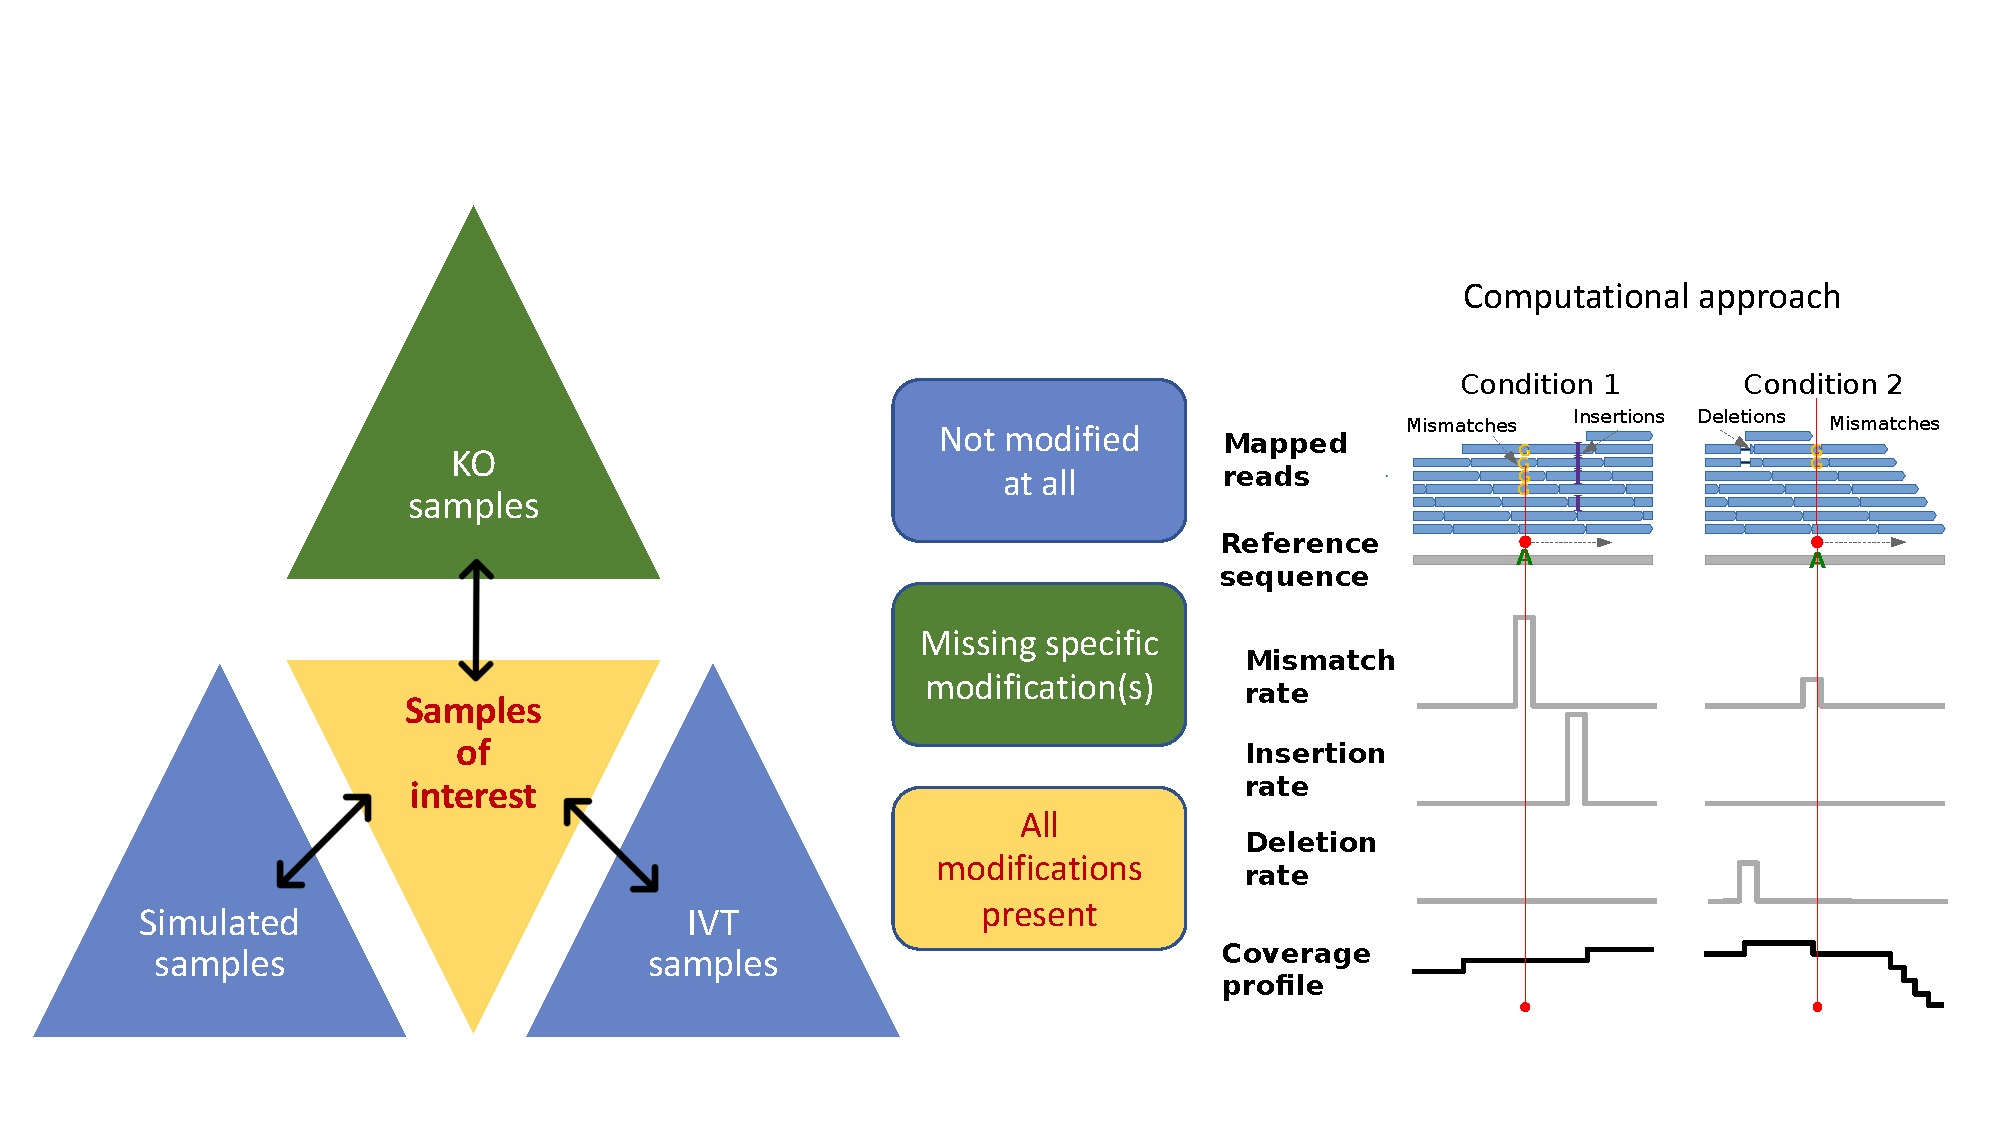
\includegraphics[width = 1\textwidth]{Figure1.pdf}
  \caption{\textbf{General outline of RNA modification detection by JACUSA2.} A key feature of our approach is that multiple replicates can be compared as shown on the left. Samples of interests where all modifications are present could be compared with either KO samples where the modification of interest is missing or IVT/simulated samples where all modifications are absent. Read stacks (in blue) are compared head-to-head as shown on the right. }
  \label{fig:graphicsummary}
      \end{figure}
\newpage

\begin{figure}[h!]
    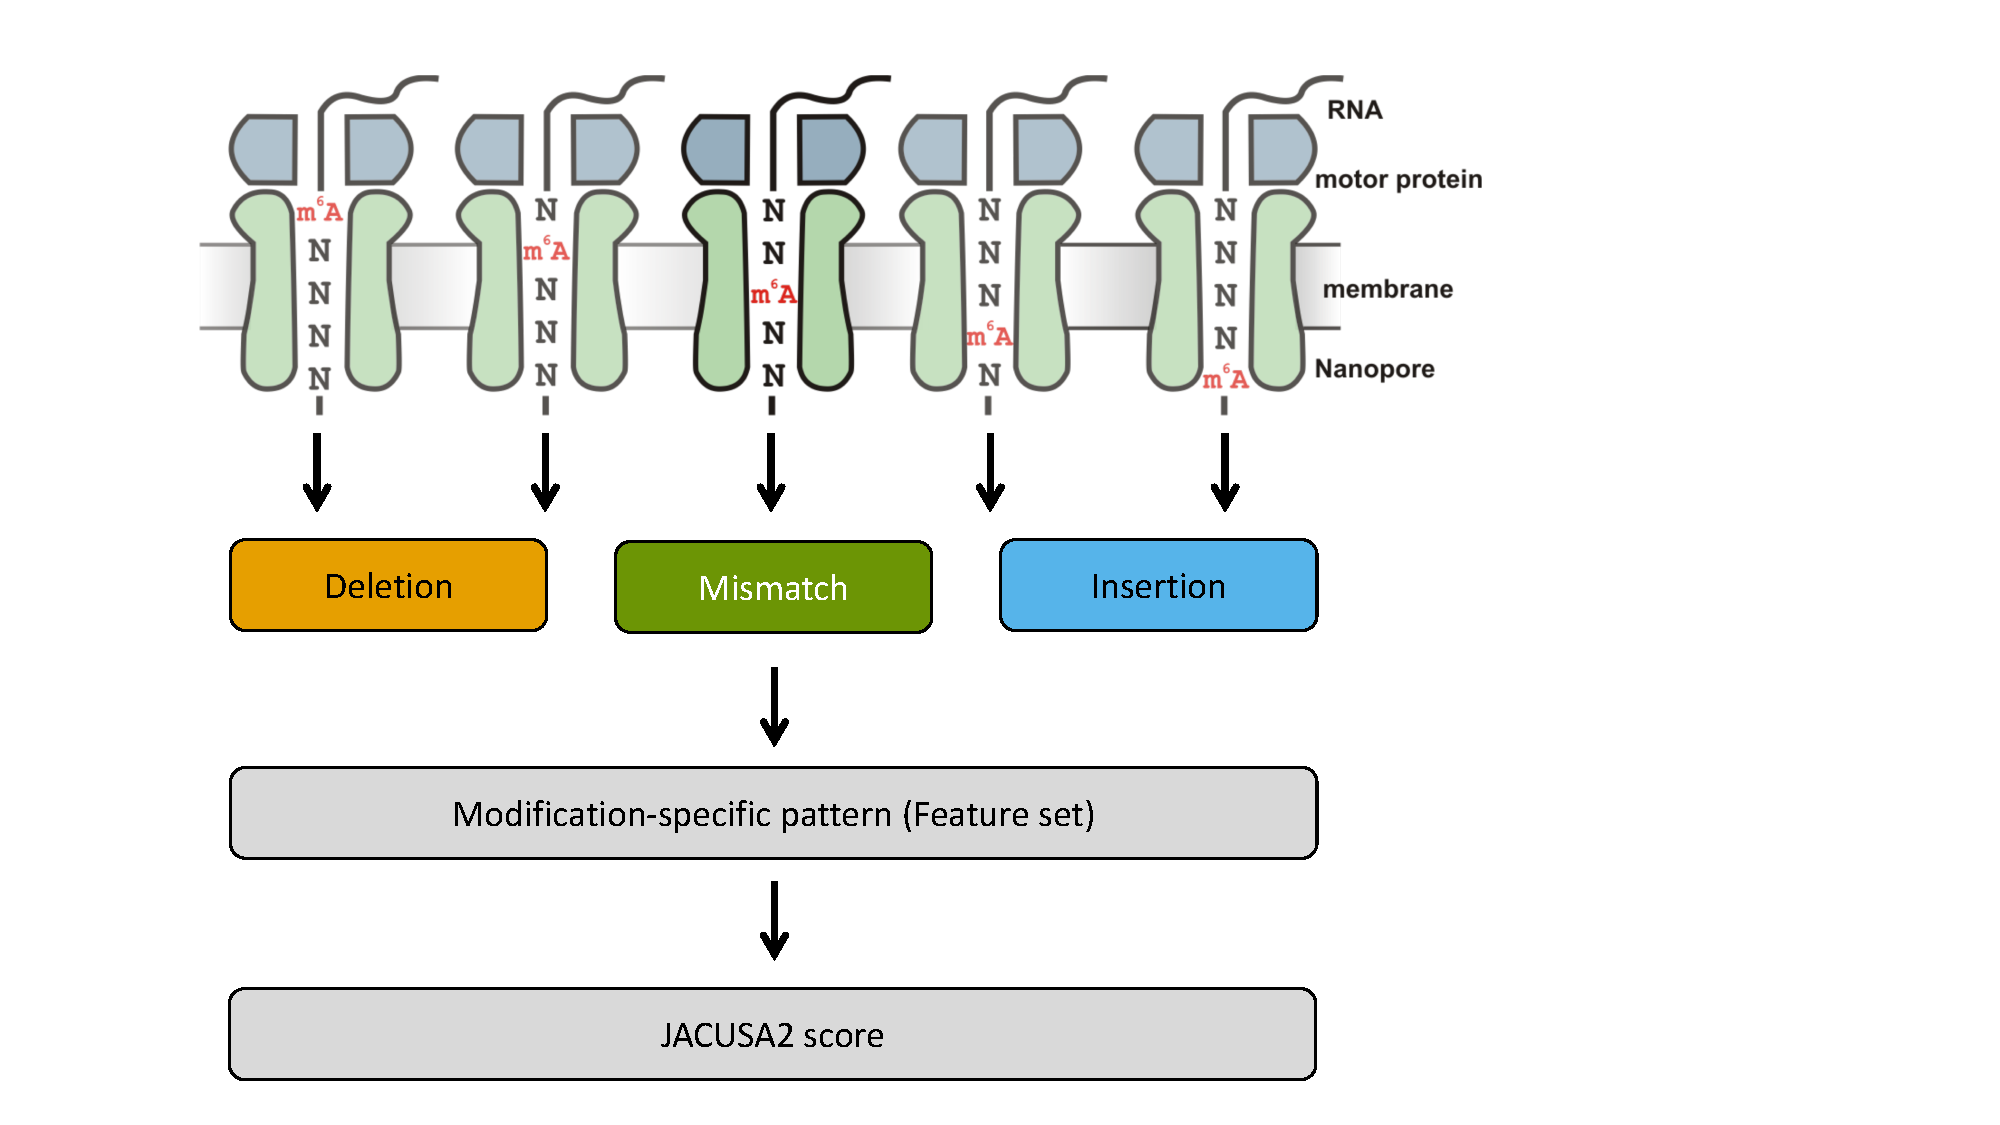
\includegraphics[width = 1\textwidth]{Figure2.pdf}
  \caption{\textbf{Motivation of 5-mer context for RNA modification mapping}. The nanopore covers 5 consecutive RNA residues. That is why we consider a 5-mer context and derive 3 principal features for every position within a given 5-mer (15 features in total, with a central A residue in this example). We evaluate each feature set by previously learned patterns and compute a final score for modification site detection.}
  \label{fig:5mer}
      \end{figure}
\newpage

\begin{figure}[h!]
    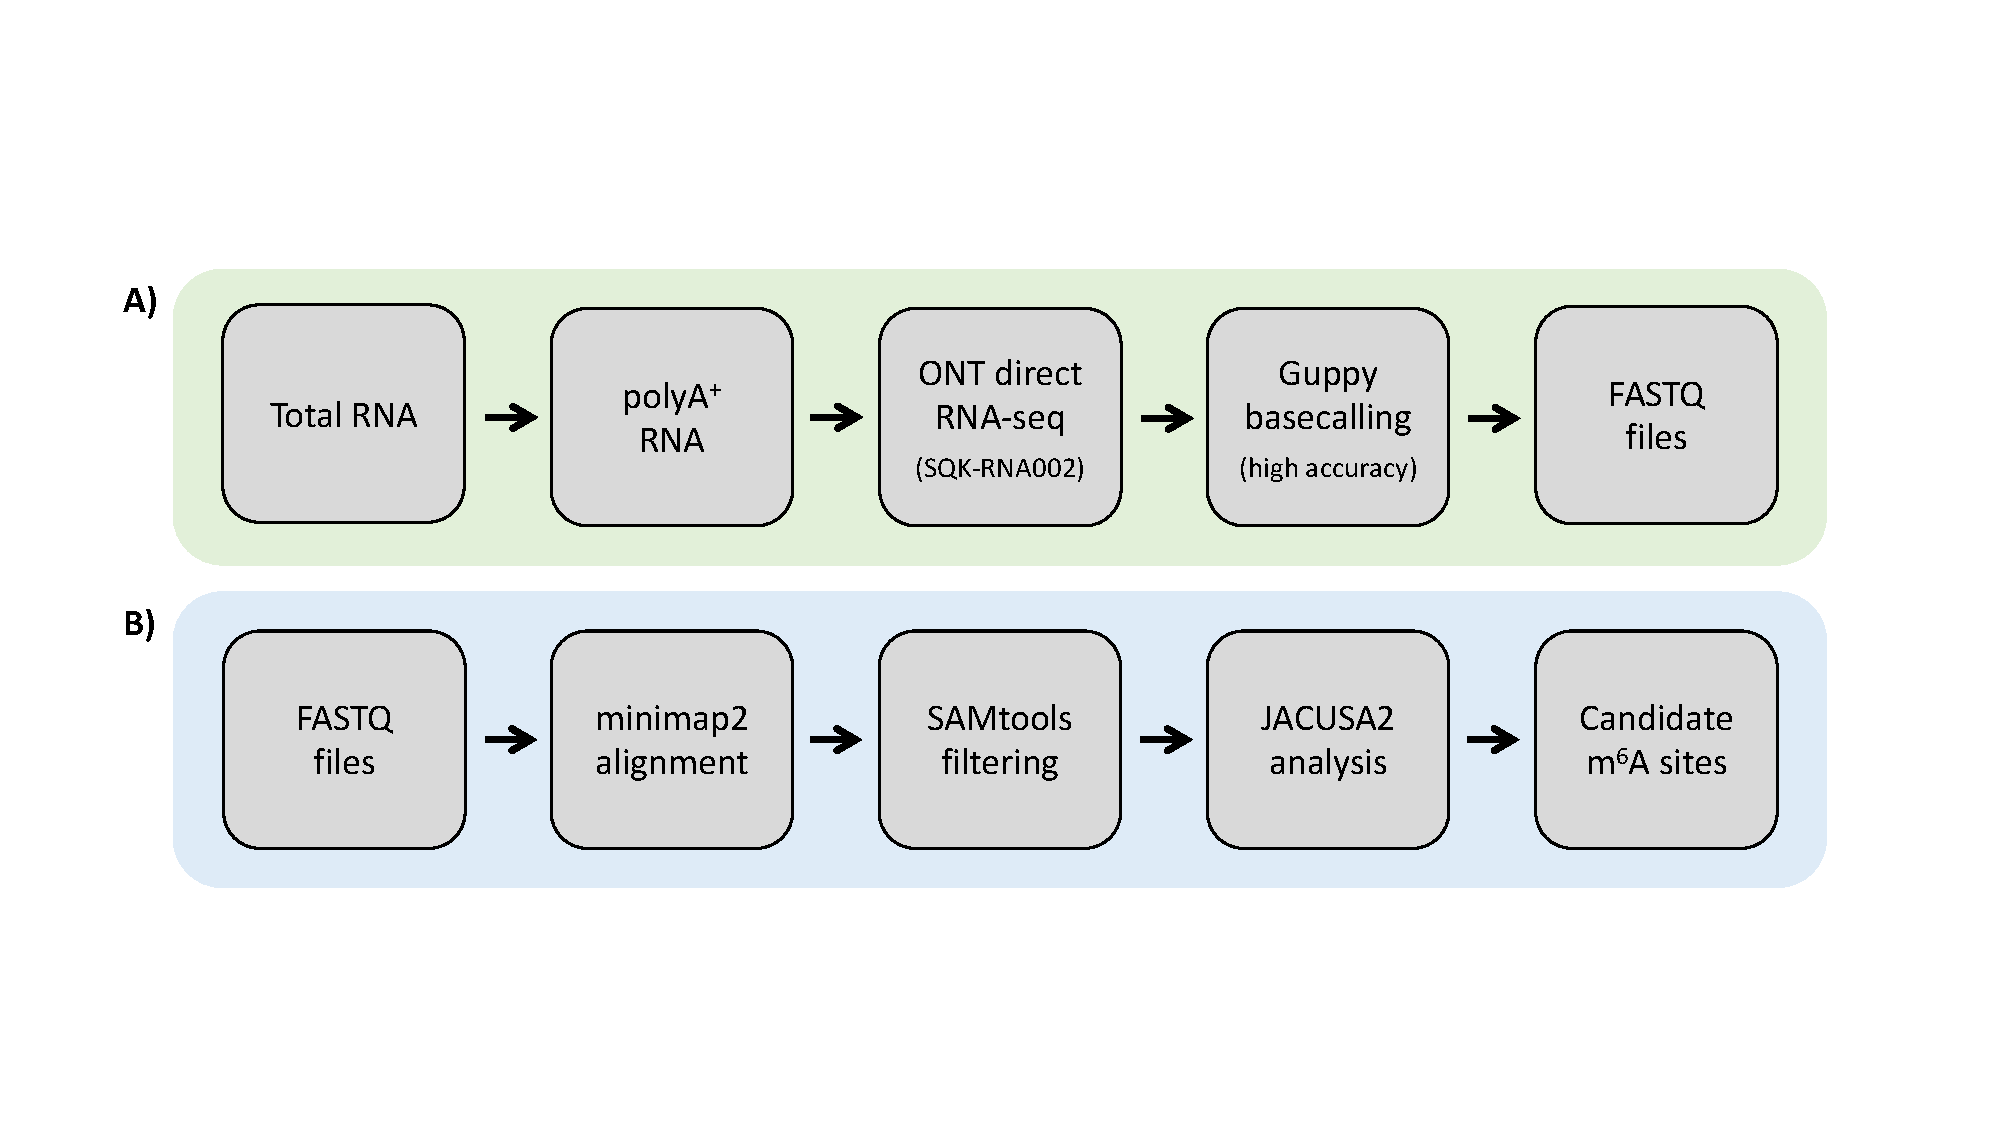
\includegraphics[width = 1\textwidth]{Figure3.pdf}
  \caption{\textbf{Experimental and computational workflow}. A) Starting from total cellular RNA, polyA\textsuperscript{+} RNA is isolated and subjected to Nanopore direct RNA-sequencing. Guppy basecalling can be done as live basecalling during sequencing or after the sequencing run from generated FAST5 files, resulting in FASTQ output files. B) FASTQ files are aligned to a reference sequence with Minimap2. SAMtools is used to generate BAM files as inpug for JACUSA2 analysis, which yields candidate m6A sites.}
  \label{fig:workflow}
      \end{figure}
\newpage

\begin{figure}[h!]
	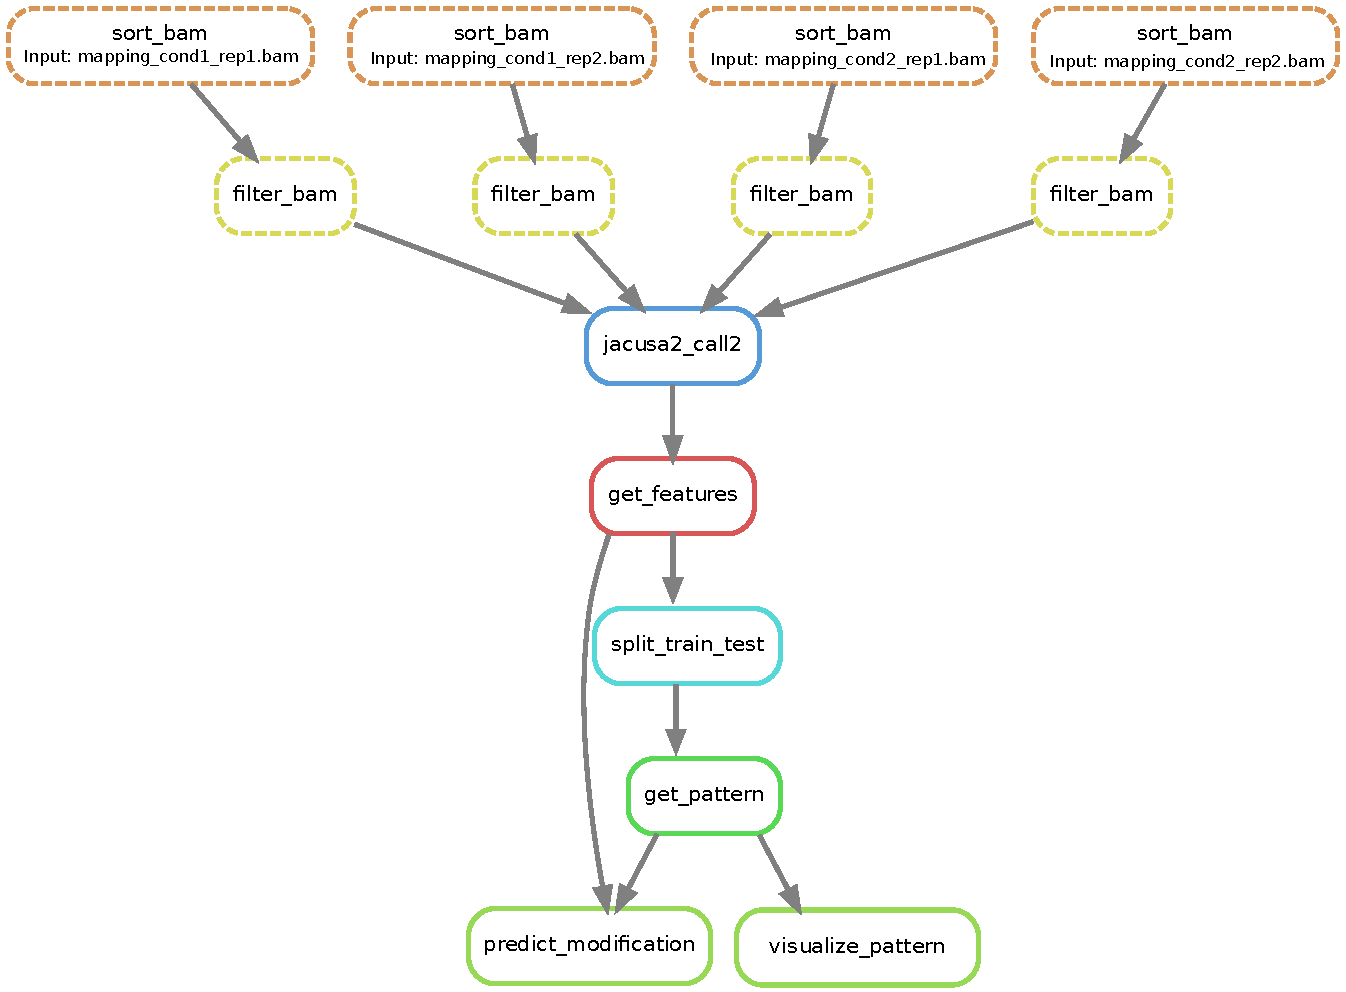
\includegraphics[width = 1\textwidth]{img/snakemake.pdf}
	\caption{\textbf{Computational workflow}. Snakemake workflow for RNA modification detection based on JACUSA2 variant calling.}
	\label{fig:snakemake}
\end{figure}
\newpage

\begin{figure}[h!]
	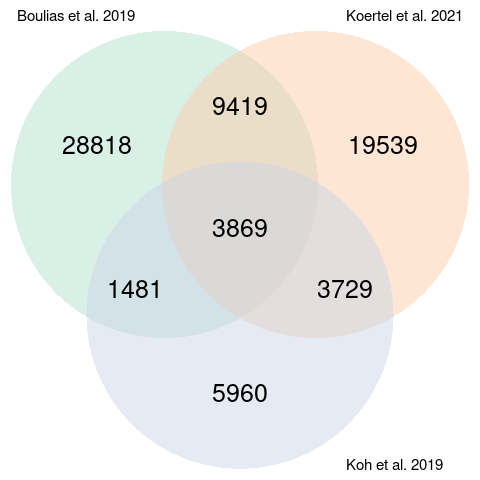
\includegraphics[width = 0.4\textwidth]{img/venn_diagramm.png}
	\caption{\textbf{m6A sites reported in the three miCLIP-based studies} Boulias et al. [2019], Koh et al. [2019] and Körtel et al. [2021].}
	\label{fig:miclip_sites}
\end{figure}
\newpage

\begin{figure}[h!]
	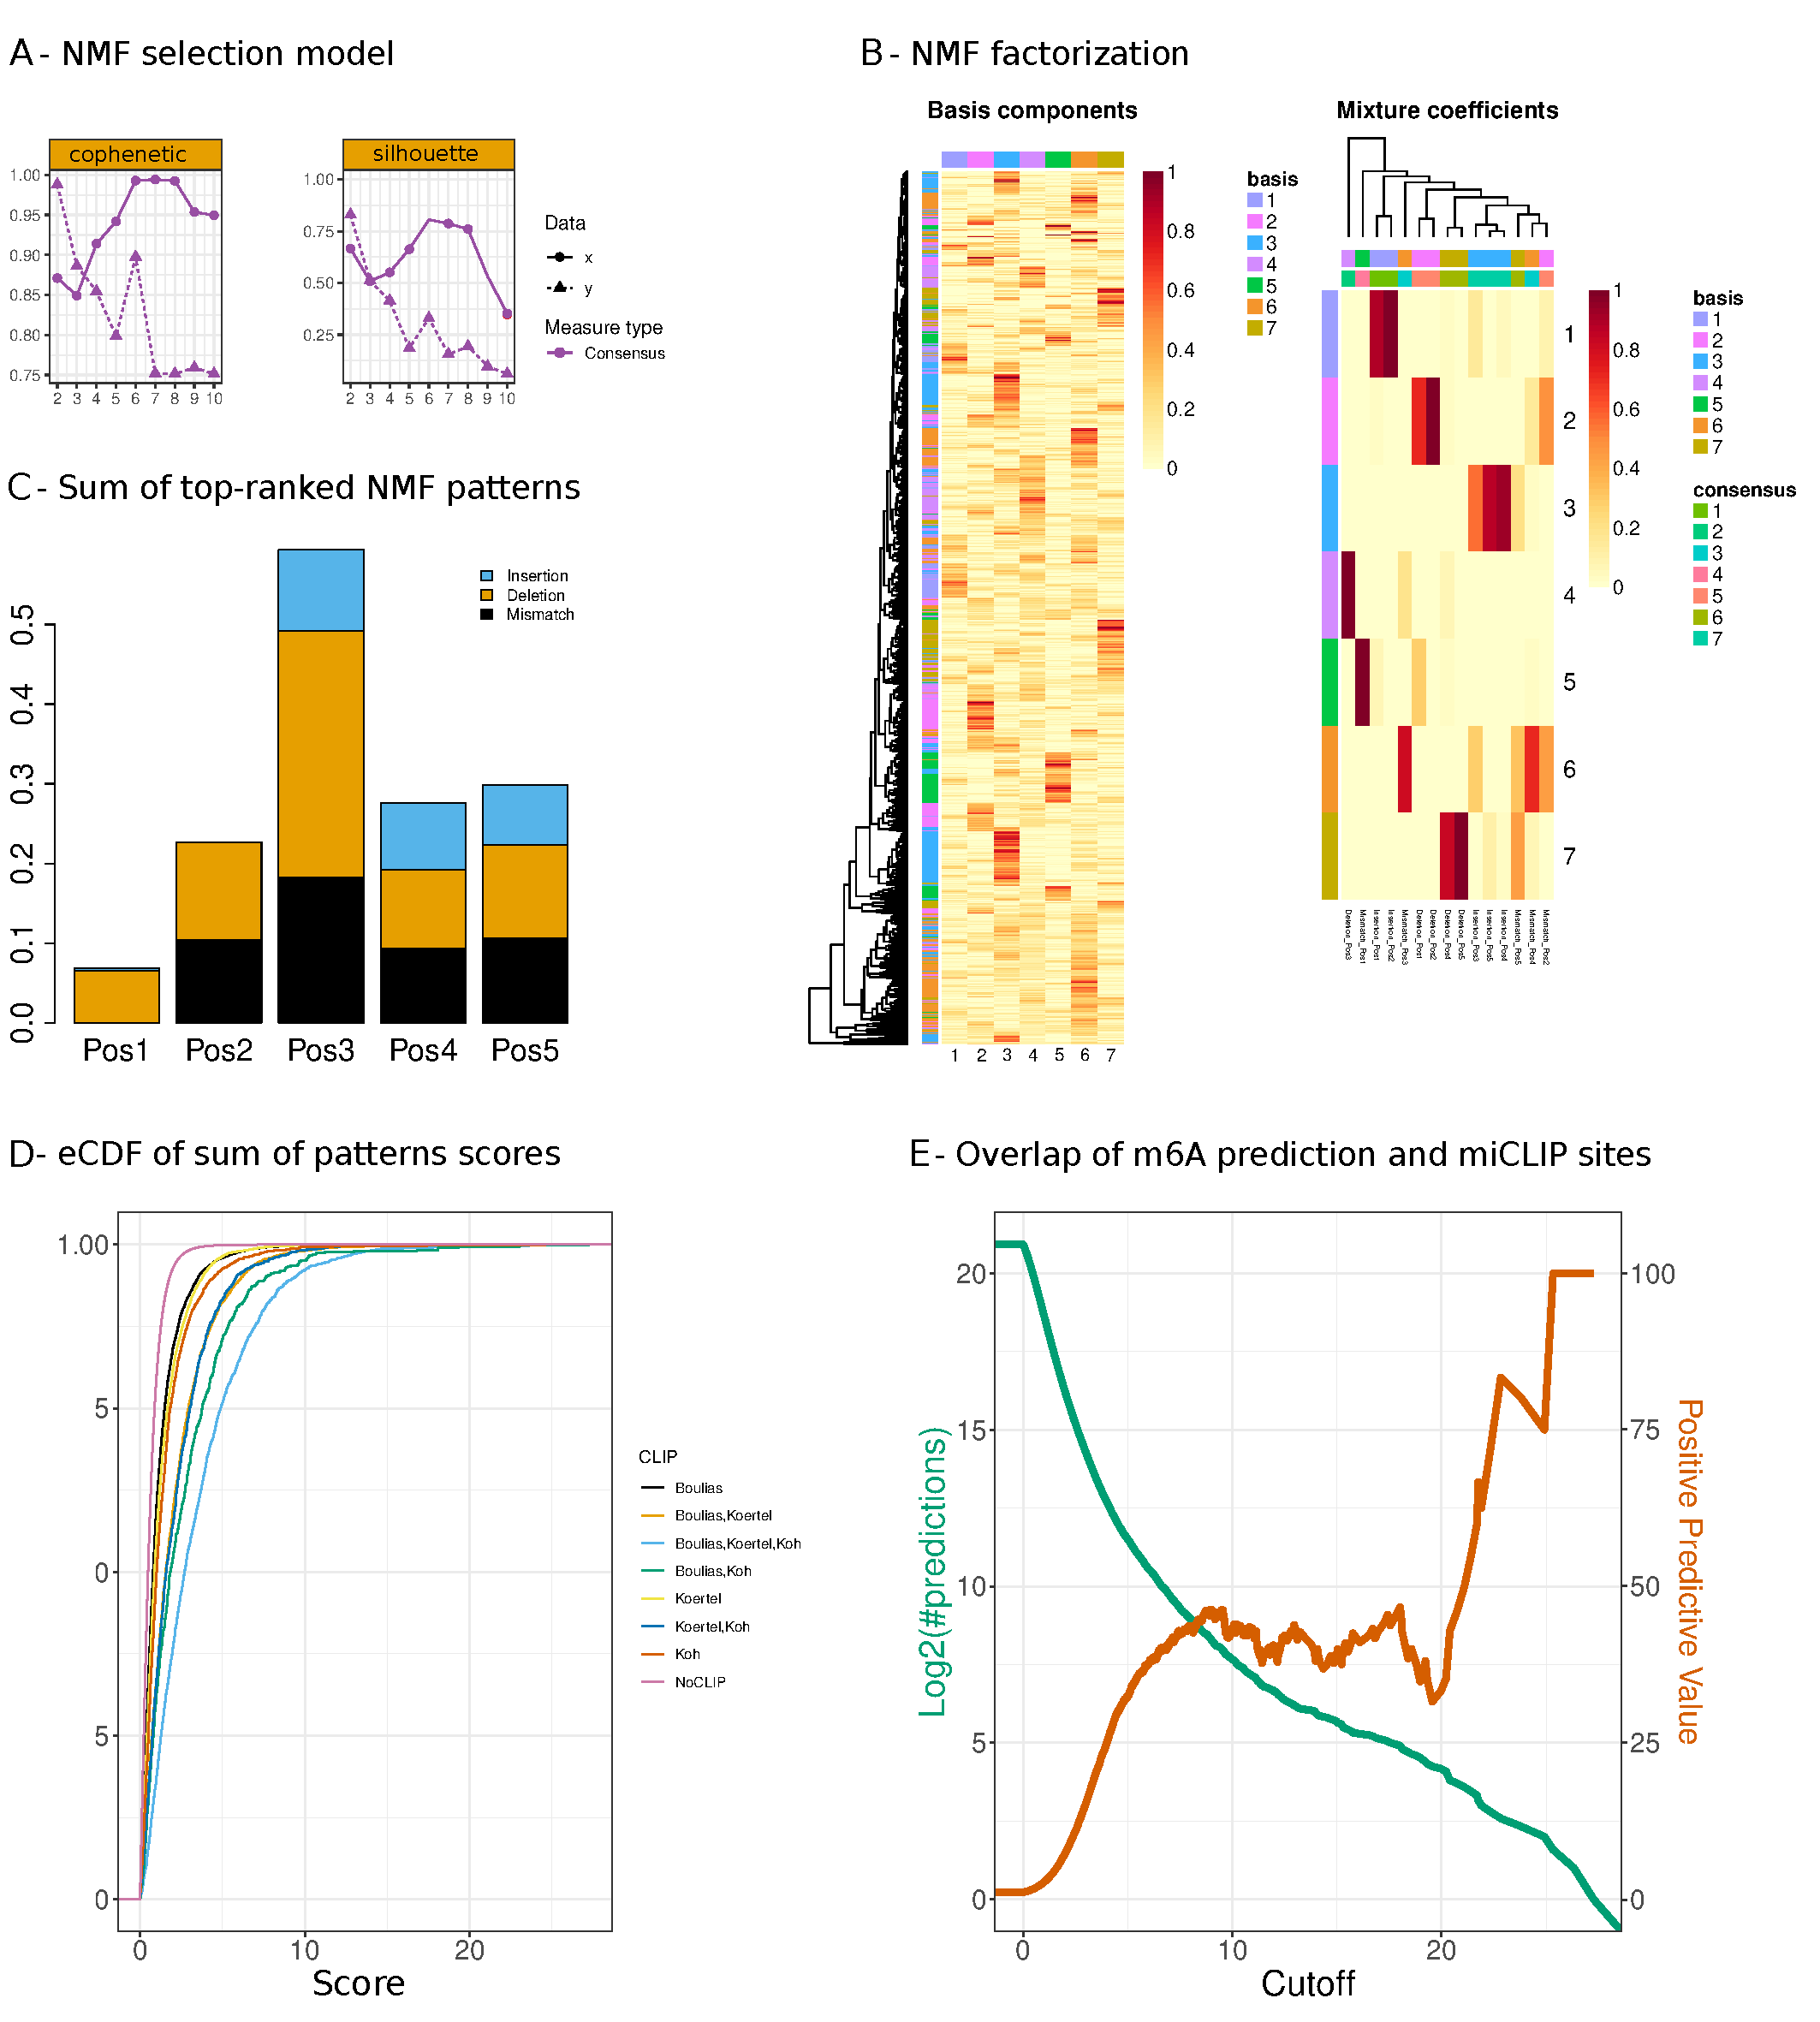
\includegraphics[width = 1\textwidth]{img/res_wt_ko.pdf}
	\caption{\textbf{Case 1. WT  versus KO.}  \textbf{A}: NMF rank selection. \textcolor{red}{Barplots representing the difference of cophenetic correlation and silhouette indices between the NMF factorization of the original and the randomized data. Ranks with the largest value for both indices are determined, then the smallest rank is selected for the NMF decomposition}. \textbf{B}: NMF result represented by the basis matrix $W$ and the coefficient matrix $H$. The matrix $H$ induces the RNA modification pattern. \textbf{C}: Barplots representing the linear combination of the top 5 patterns (y-axis) by the number of position in the specific 5-mer context (x-axis) and the score type: mismatch, deletion and insertion (resp. black, orange and blue). The 5 patterns (coefficient vectors: 1,2,3,4,6) are selected according to the predominant columns in matrix W.  \textbf{D}: Score distribution inferred from the combined patterns, stratified by the different categories of miCLIP validated sites and non miCLIP sites.  \textbf{E}: Number of predicted m6A sites (green) and Positive Predictive Value (PPV) of predicted m6A sites that overlap with miCLIP sites (orange). }
	\label{fig:WT_KO}
\end{figure}

\newpage
\begin{figure}[h!]
	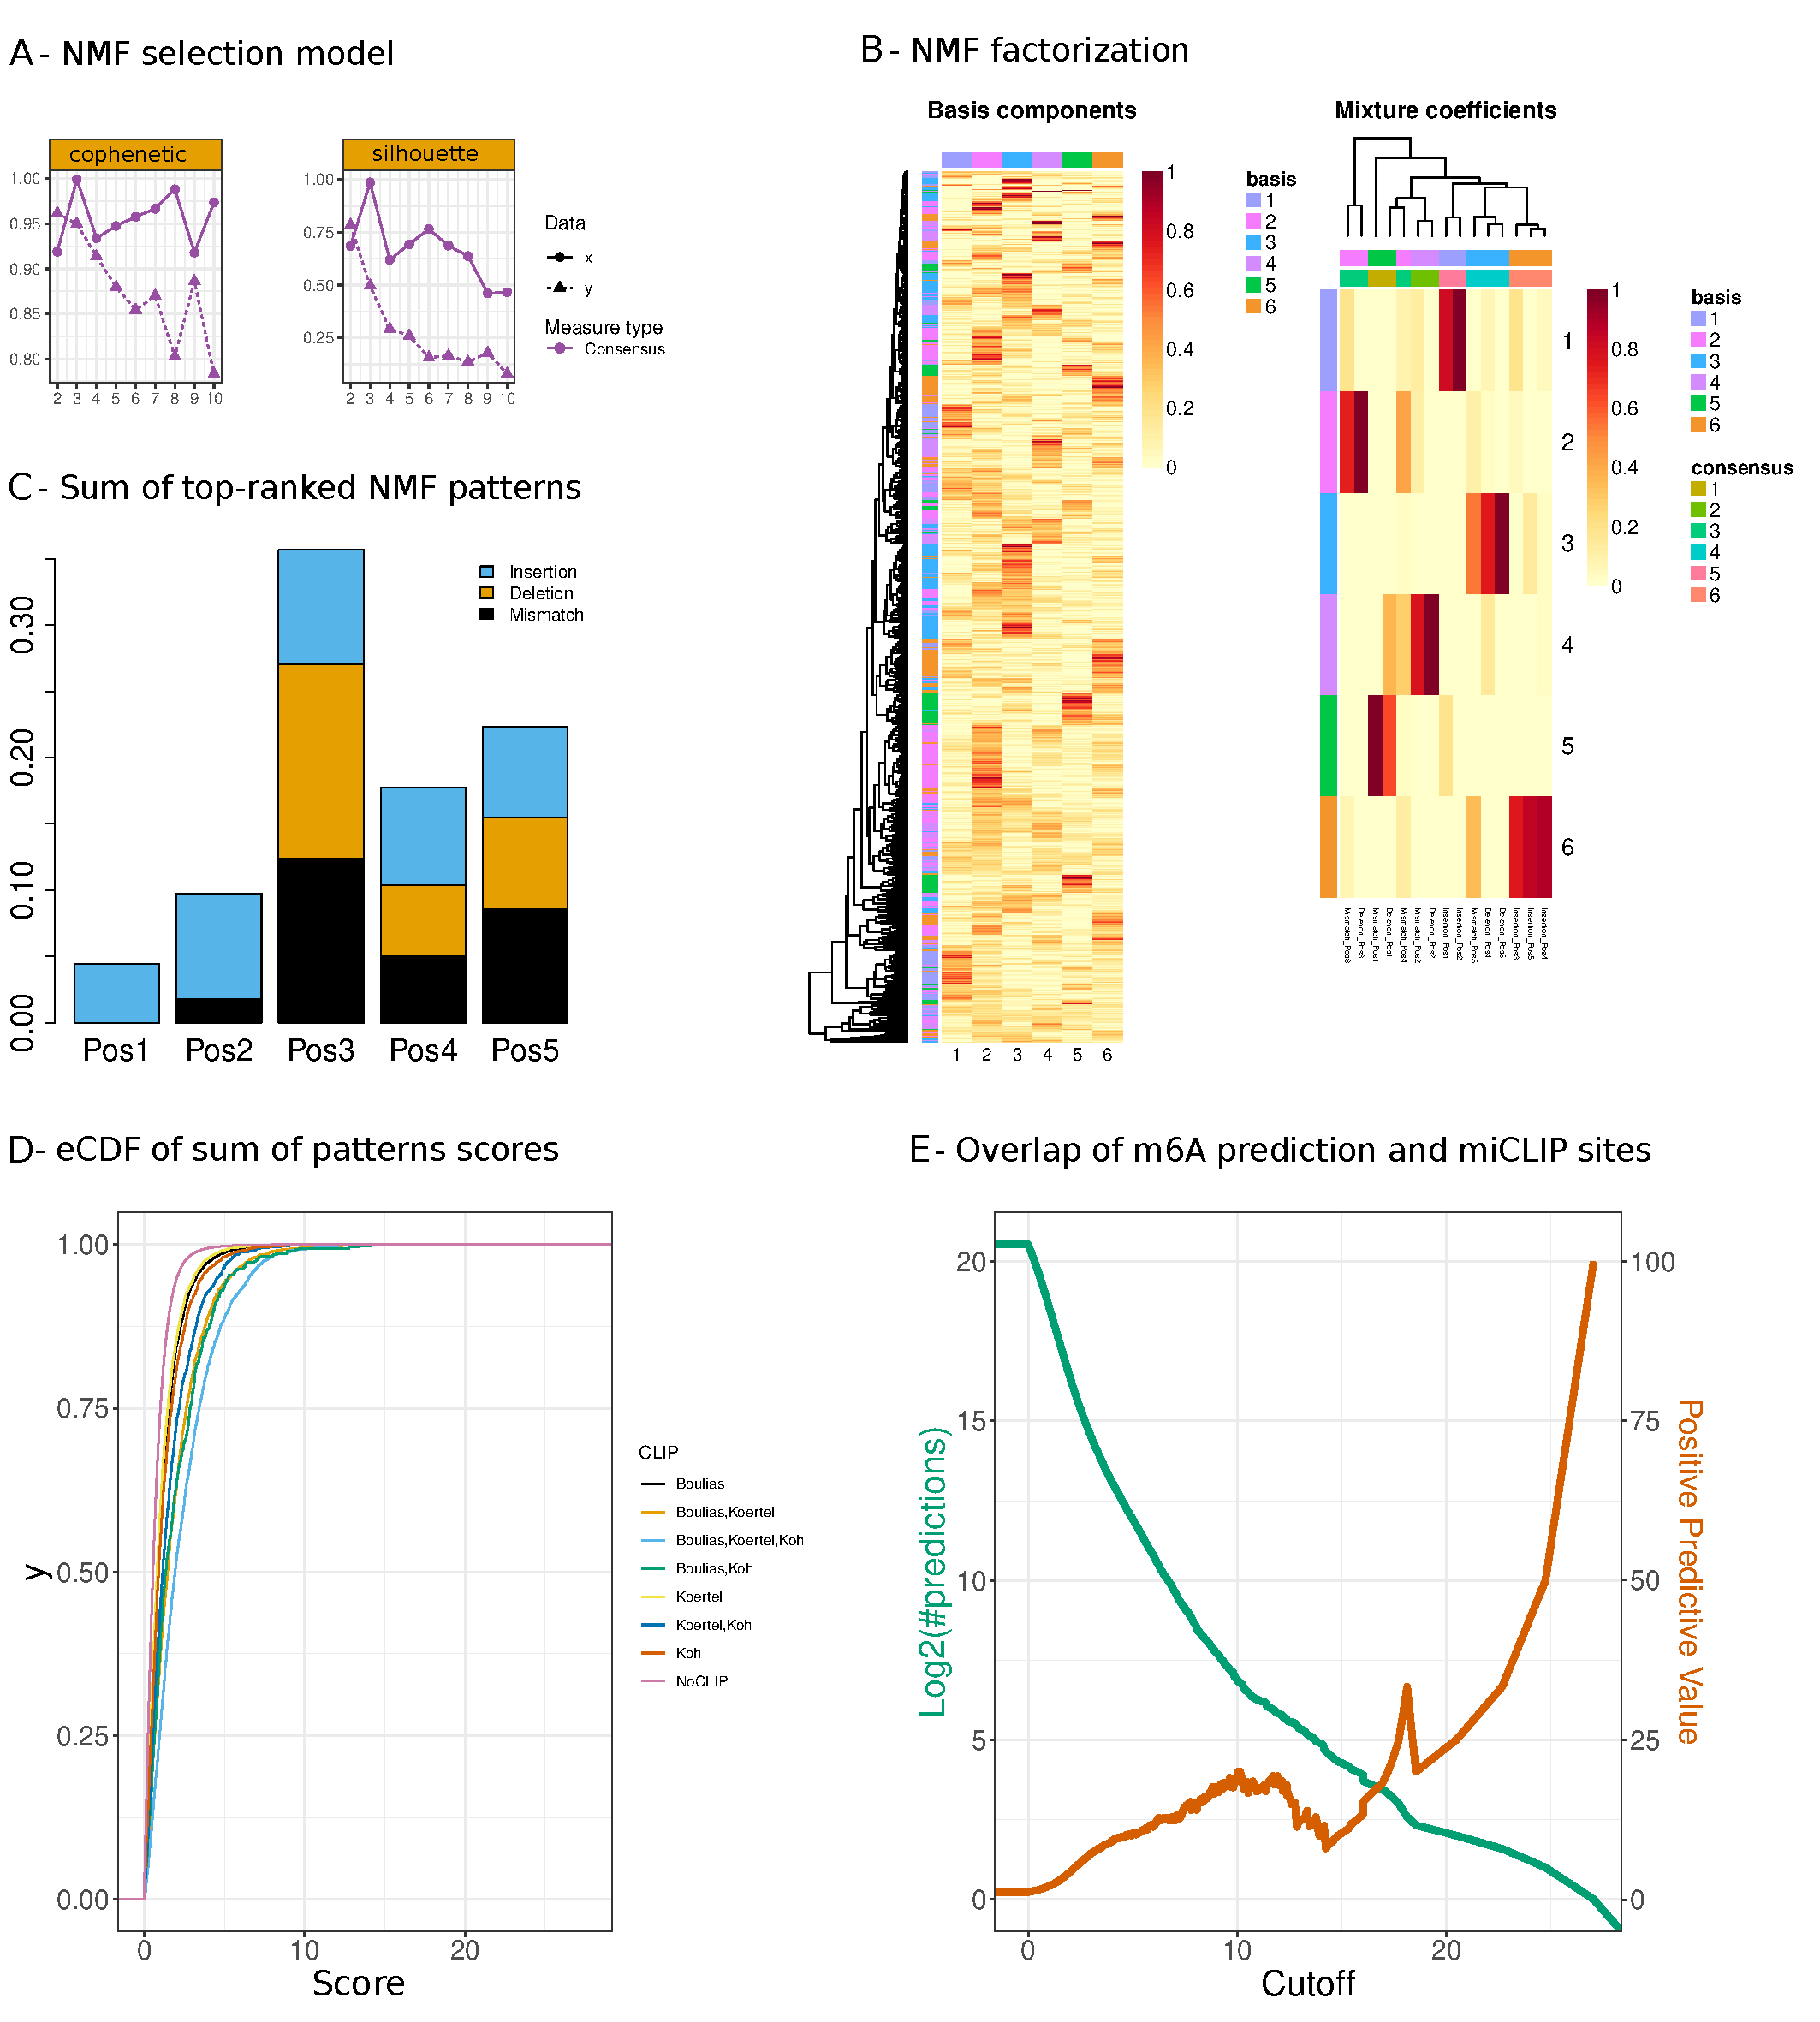
\includegraphics[width = 1\textwidth]{img/res_wt_ivt.pdf}
	\caption{\textbf{Case 2. WT  versus IVT.}  \textbf{A}: NMF rank selection. \textcolor{red}{Barplots representing the difference of cophenetic correlation and silhouette indices between the NMF factorization of the original and the randomized data. Ranks with the largest value for both indices are determined, then the smallest rank is selected for the NMF decomposition.} \textbf{B}: NMF result represented by the basis matrix $W$ and the coefficient matrix $H$. The matrix $H$ induces the RNA modification pattern. \textbf{C}: Barplots representing the linear combination of the top 4 patterns (y-axis) by by the number of position in the specific 5-mer context (x-axis) and the score type: mismatch, deletion and insertion (resp. black, orange and blue). The 4 patterns (coefficient vectors: 1,2,3,6) are selected according to the predominant columns in matrix W.  \textbf{D}: Score distribution inferred from the combined patterns, stratified by the different categories of miCLIP validated sites and non miCLIP sites.  \textbf{E}: Number of predicted m6A sites (green) and Positive Predictive Value (PPV) of predicted m6A sites that overlap with miCLIP sites (orange). }
	\label{fig:WT_IVT}
\end{figure}
\newpage
\section*{TABLE CAPTIONS}
\section*{TABLES}

\begin{table}[]
\label{tab:software}
\begin{tabular}{|p{1.5cm}|p{7cm}|p{6.5cm}|}
\hline 
            Software & Version & Description \\ 
            \hline \hline
            \texttt{Minimap2} & \url{https://github.com/lh3/minimap2} v2.22 or later & \url{https://lh3.github.io/minimap2/} \\ \hline
            \texttt{samtools} & \url{https://github.com/samtools/samtools} v1.12 or later & \url{http://samtools.github.io/} \\ \hline
	   \texttt{JAVA} & \url{https://openjdk.java.net/} 11.0.12 2021-07-20 - JAVA 11 or later & OpenJDK Runtime Environment\\ \hline
	   \texttt{R} &  \url{https://www.r-project.org/} version 3.5.1 or later & The R Project for Statistical Computing \\ \hline
	   \texttt{PERL} &  \url{https://www.perl.org/} version 5.28.1 or later & Perl is a highly capable, feature-rich programming language \\ \hline
	   \texttt{bedtools} &  \url{https://github.com/arq5x/bedtools2} version 2.29.2 or later & Perl is a highly capable, feature-rich programming language \\ \hline	   
	   \texttt{snakemake} &  \url{https://snakemake.github.io/} version 6.8.1 or later & The Snakemake workflow management system\\ \hline	   
\end{tabular}
\caption{\textbf{Software dependencies}\label{tab:software}}
\end{table}

%Minimap2	2.22
%samtools	1.12
%openjdk	11.0.13
%R	4.0.5
%PERL	5.28.1
%bedtools	2.29.2
snakemake	6.8.1

\begin{table}[]
\label{tab:packages}
\begin{tabular}{|p{1.5cm}|p{7cm}|p{6.5cm}|}
\hline 
            R Packages & Version & Description \\ 
            \hline \hline
            \texttt{ggplot2} & \url{https://cran.r-project.org/web/packages/ggplot2/index.html} - ggplot2\_3.3.0 or later &  ggplot2 is a system for declaratively creating graphics, based on The Grammar of Graphics. \\ \hline
            \texttt{NMF} & \url{https://cran.r-project.org/web/packages/NMF/index.html} - NMF\_0.22.0 or later &  Provides a framework to perform Non-negative Matrix Factorization (NMF). \\ \hline
\end{tabular}
\caption{\textbf{R Package dependencies}\label{tab:software}}
\end{table}



\end{document}
